% =============================================================================
%  LogiFlow --- Articulo IEEE (Release 2)
%  Arquitecturas de Software --- ECI Julio Garavito --- Mayo 2026
%  Estilo oficial: IEEEtran (conference)
% =============================================================================
\documentclass[conference]{IEEEtran}
\IEEEoverridecommandlockouts

% --- Codificacion e idioma ----------------------------------------------------
\usepackage[utf8]{inputenc}
\usepackage[T1]{fontenc}
\usepackage[spanish,es-tabla]{babel}
\usepackage{lmodern}

% --- Paquetes estandar para IEEE ----------------------------------------------
\usepackage{cite}
\usepackage{amsmath,amssymb,amsfonts}
\usepackage{graphicx}
\usepackage{textcomp}
\usepackage{xcolor}
\usepackage{url}
\usepackage{booktabs}
\usepackage{array}
\usepackage{tabularx}
\usepackage{hyperref}

% --- Configuracion de hyperref para IEEE --------------------------------------
\hypersetup{
  colorlinks=true,
  linkcolor=blue!50!black,
  citecolor=blue!50!black,
  urlcolor=blue!50!black,
  pdftitle={LogiFlow: Plataforma distribuida cloud-native para ruteo dinamico de flotas en tiempo real},
  pdfauthor={Sanchez Mendez, Pedraza Rodriguez, Correa Suarez, Ortega Munoz}
}

% --- Listings minimal para snippets de codigo ---------------------------------
\usepackage{listings}
\lstset{
  basicstyle=\ttfamily\scriptsize,
  breaklines=true,
  showstringspaces=false,
  columns=flexible
}

\def\BibTeX{{\rm B\kern-.05em{\sc i\kern-.025em b}\kern-.08em T\kern-.1667em\lower.7ex\hbox{E}\kern-.125emX}}

% =============================================================================
\begin{document}

% =============================================================================
% TITULO Y AUTORES
% =============================================================================
\title{LogiFlow: Plataforma distribuida \emph{cloud-native} para ruteo din\'amico de flotas en tiempo real bajo un enfoque de microservicios y atributos de calidad medidos en producci\'on}

\author{
\IEEEauthorblockN{Andersson David S\'anchez M\'endez}
\IEEEauthorblockA{\textit{Ingenier\'ia de Sistemas} \\
\textit{Escuela Colombiana de Ingenier\'ia Julio Garavito}\\
Bogot\'a, Colombia \\
andersson.sanchez-m@mail.escuelaing.edu.co}
\and
\IEEEauthorblockN{Cristian Santiago Pedraza Rodr\'iguez}
\IEEEauthorblockA{\textit{Ingenier\'ia de Sistemas} \\
\textit{Escuela Colombiana de Ingenier\'ia Julio Garavito}\\
Bogot\'a, Colombia \\
cristian.pedraza-m@mail.escuelaing.edu.co}
\and
\IEEEauthorblockN{Elizabeth Correa Su\'arez}
\IEEEauthorblockA{\textit{Ingenier\'ia de Sistemas} \\
\textit{Escuela Colombiana de Ingenier\'ia Julio Garavito}\\
Bogot\'a, Colombia \\
elizabeth.correa-s@mail.escuelaing.edu.co}
\and
\IEEEauthorblockN{Juan Sebasti\'an Ortega Mu\~noz}
\IEEEauthorblockA{\textit{Ingenier\'ia de Sistemas} \\
\textit{Escuela Colombiana de Ingenier\'ia Julio Garavito}\\
Bogot\'a, Colombia \\
juan.ortega-m@mail.escuelaing.edu.co}
}

\maketitle

% =============================================================================
% RESUMEN
% =============================================================================
\begin{abstract}
Este art\'iculo presenta \emph{LogiFlow}, una plataforma distribuida \emph{cloud-native} dise\~nada para resolver el \emph{Vehicle Routing Problem} (VRP) din\'amico en menos de cuatro segundos ante eventos de tr\'afico, cierres viales o incidencias log\'isticas. La soluci\'on adopta un estilo arquitect\'onico basado en microservicios con un \emph{API Gateway} sobre NestJS, optimizaci\'on gRPC contra VROOM, ajuste de matrices de duraci\'on mediante un modelo de IA propio para corredores de Bogot\'a, comunicaci\'on en tiempo real con \emph{Socket.io} respaldada por \emph{Redis Pub/Sub}, automatizaci\'on de ingesta de eventos con \emph{n8n} y notificaciones multicanal con \emph{OpenClaw} y \emph{Firebase Cloud Messaging}. El sistema fue desplegado en producci\'on sobre Azure con infraestructura como c\'odigo (Terraform). Los resultados medidos sobre el entorno real reportan \textbf{20.98~TPS} sostenibles con P95 de \textbf{2.8 segundos} bajo 50 usuarios concurrentes, \textbf{99.79\%} de disponibilidad de infraestructura, \textbf{cobertura de tests} de 80.49\% en frontend y 83.36\% en backend, y portabilidad total mediante Docker y Terraform.
\end{abstract}

\begin{IEEEkeywords}
arquitectura de software, microservicios, Vehicle Routing Problem, gRPC, WebSocket, atributos de calidad, escalabilidad, IEEE 1471
\end{IEEEkeywords}

% =============================================================================
% I. INTRODUCCION
% =============================================================================
\section{Introducci\'on}

La log\'istica urbana en Latinoam\'erica enfrenta ineficiencias estructurales. Cerca del \textbf{23\%} de las entregas de \'ultima milla llegan con retraso y se estima que el \textbf{40\%} de los costos operacionales se generan por ruteo sub\'optimo evitable. La causa ra\'iz suele ser la incapacidad del sistema log\'istico de reaccionar en tiempo real ante eventos imprevistos como cierres viales, accidentes o cambios en las \'ordenes. Cuando una v\'ia se cierra a mitad de la jornada, los conductores siguen la ruta original, llegan tarde y el cliente no vuelve.

\emph{LogiFlow} aborda este problema con una plataforma distribuida \emph{cloud-native} que cierra el ciclo entre la detecci\'on del evento, la reoptimizaci\'on del VRP y la entrega de la nueva ruta a cada conductor. El alcance cubre dos monorepos. Por un lado, un backend con nueve servicios contenedorizados: \emph{gateway, realtime, optimizer, vroom, ai-predictor, n8n, openclaw, postgres} y \emph{redis}. Por el otro, un frontend con dos aplicaciones Angular, una \emph{web-admin} para despachadores y una \emph{mobile} construida con Ionic y Capacitor para conductores, m\'as cuatro librer\'ias TypeScript compartidas.

La motivaci\'on t\'ecnica fue construir un sistema que sirviera como banco de pruebas real para los cuatro atributos de calidad exigidos por la asignatura (disponibilidad, seguridad, mantenibilidad y portabilidad), y para un objetivo de rendimiento concreto: que el ciclo evento--ruta entregada se completara en menos de cuatro segundos. El sistema completo est\'a desplegado y operativo en \url{https://logiflowapp.z13.web.core.windows.net}.

Este art\'iculo documenta la arquitectura, la metodolog\'ia, los logros t\'ecnicos y los resultados medidos. La Secci\'on~\ref{sec:metodologia} describe el enfoque Scrum. La Secci\'on~\ref{sec:arquitectura} presenta la arquitectura y las decisiones clave. La Secci\'on~\ref{sec:logros} detalla los logros por cada atributo de calidad. La Secci\'on~\ref{sec:resultados} muestra los resultados num\'ericos. La Secci\'on~\ref{sec:conclusiones} cierra con limitaciones y trabajo futuro.

% =============================================================================
% II. METODOLOGIA
% =============================================================================
\section{Metodolog\'ia}
\label{sec:metodologia}

El proyecto se desarroll\'o bajo \textbf{Scrum} \cite{scrum-guide} con sprints de dos semanas y \textbf{Azure DevOps} como herramienta oficial de gesti\'on del \emph{Product Backlog}, el \emph{Sprint Backlog} y el \emph{Burndown Chart}. Las ceremonias estandarizadas fueron Sprint Planning, Daily as\'incrono v\'ia Discord (por horarios de clase disjuntos entre los integrantes), Sprint Review con demo en vivo y Sprint Retrospective en formato \emph{Mad/Sad/Glad}.

Los criterios de \emph{Definition of Ready} exigen que toda historia tenga formato \emph{Como [rol] quiero [acci\'on]}, criterios de aceptaci\'on enumerados, estimaci\'on Fibonacci consensuada y dependencias declaradas. Los criterios de \emph{Definition of Done} requieren c\'odigo \emph{merged} a \texttt{main} v\'ia \emph{pull request} con CI en verde (lint, tests, cobertura $\geq 80\%$), demo realizada y, si la historia afecta producci\'on, despliegue validado con \emph{smoke test}.

La planificaci\'on inicial contemplaba siete sprints, pero la curva de aprendizaje en tecnolog\'ias nuevas para el equipo (gRPC, Terraform, Google OAuth, Firebase Cloud Messaging, \emph{Socket.io} con \emph{Redis Pub/Sub}) extendi\'o el proceso a \textbf{10 sprints reales} con \textbf{245 puntos de historia entregados}. Los hitos principales fueron: \emph{S1 MVP Conectado} (13~pts), \emph{S2 APIs Reales} (21~pts), \emph{S3 Optimizer Vivo} (21~pts), \emph{S4 Interfaces+Auth} (34~pts), \emph{S5 Cloud Deploy Azure} (46~pts, Corte~2), \emph{S6 Observabilidad+Tests} (34~pts), \emph{S7 Escala/Performance} (21~pts) y \emph{S8 a S10 OAuth+FCM+Hardening} (55~pts, Corte~3).

GitHub se us\'o para los dos repositorios con \emph{branch protection} sobre \texttt{main} y \texttt{develop}. Esto signific\'o que ning\'un cambio entr\'o a estas ramas sin \emph{pull request} aprobado y CI en verde. La trazabilidad de cada \emph{commit} a una historia de usuario en Azure DevOps fue obligatoria.

% =============================================================================
% III. ARQUITECTURA DEL SISTEMA
% =============================================================================
\section{Arquitectura del Sistema}
\label{sec:arquitectura}

\subsection{Estilo arquitect\'onico}

LogiFlow combina cuatro estilos. El primero es \emph{microservicios}, con nueve contenedores Docker de responsabilidad \'unica. El segundo es \emph{API Gateway}, donde el servicio NestJS centraliza la autenticaci\'on y orquesta las llamadas internas. El tercero es \emph{event-driven publish/subscribe}, usando Redis Pub/Sub como bus de eventos para el Realtime Service. El cuarto es \emph{layered architecture} dentro de cada microservicio, siguiendo el patr\'on Controller~$\rightarrow$~Service~$\rightarrow$~Repository.

\subsection{Componentes clave}

La Fig.~\ref{fig:flujo} ilustra el flujo de un evento de tr\'afico desde la fuente externa hasta el cliente. Los componentes y sus roles son los siguientes:

\begin{figure}[ht]
\centering
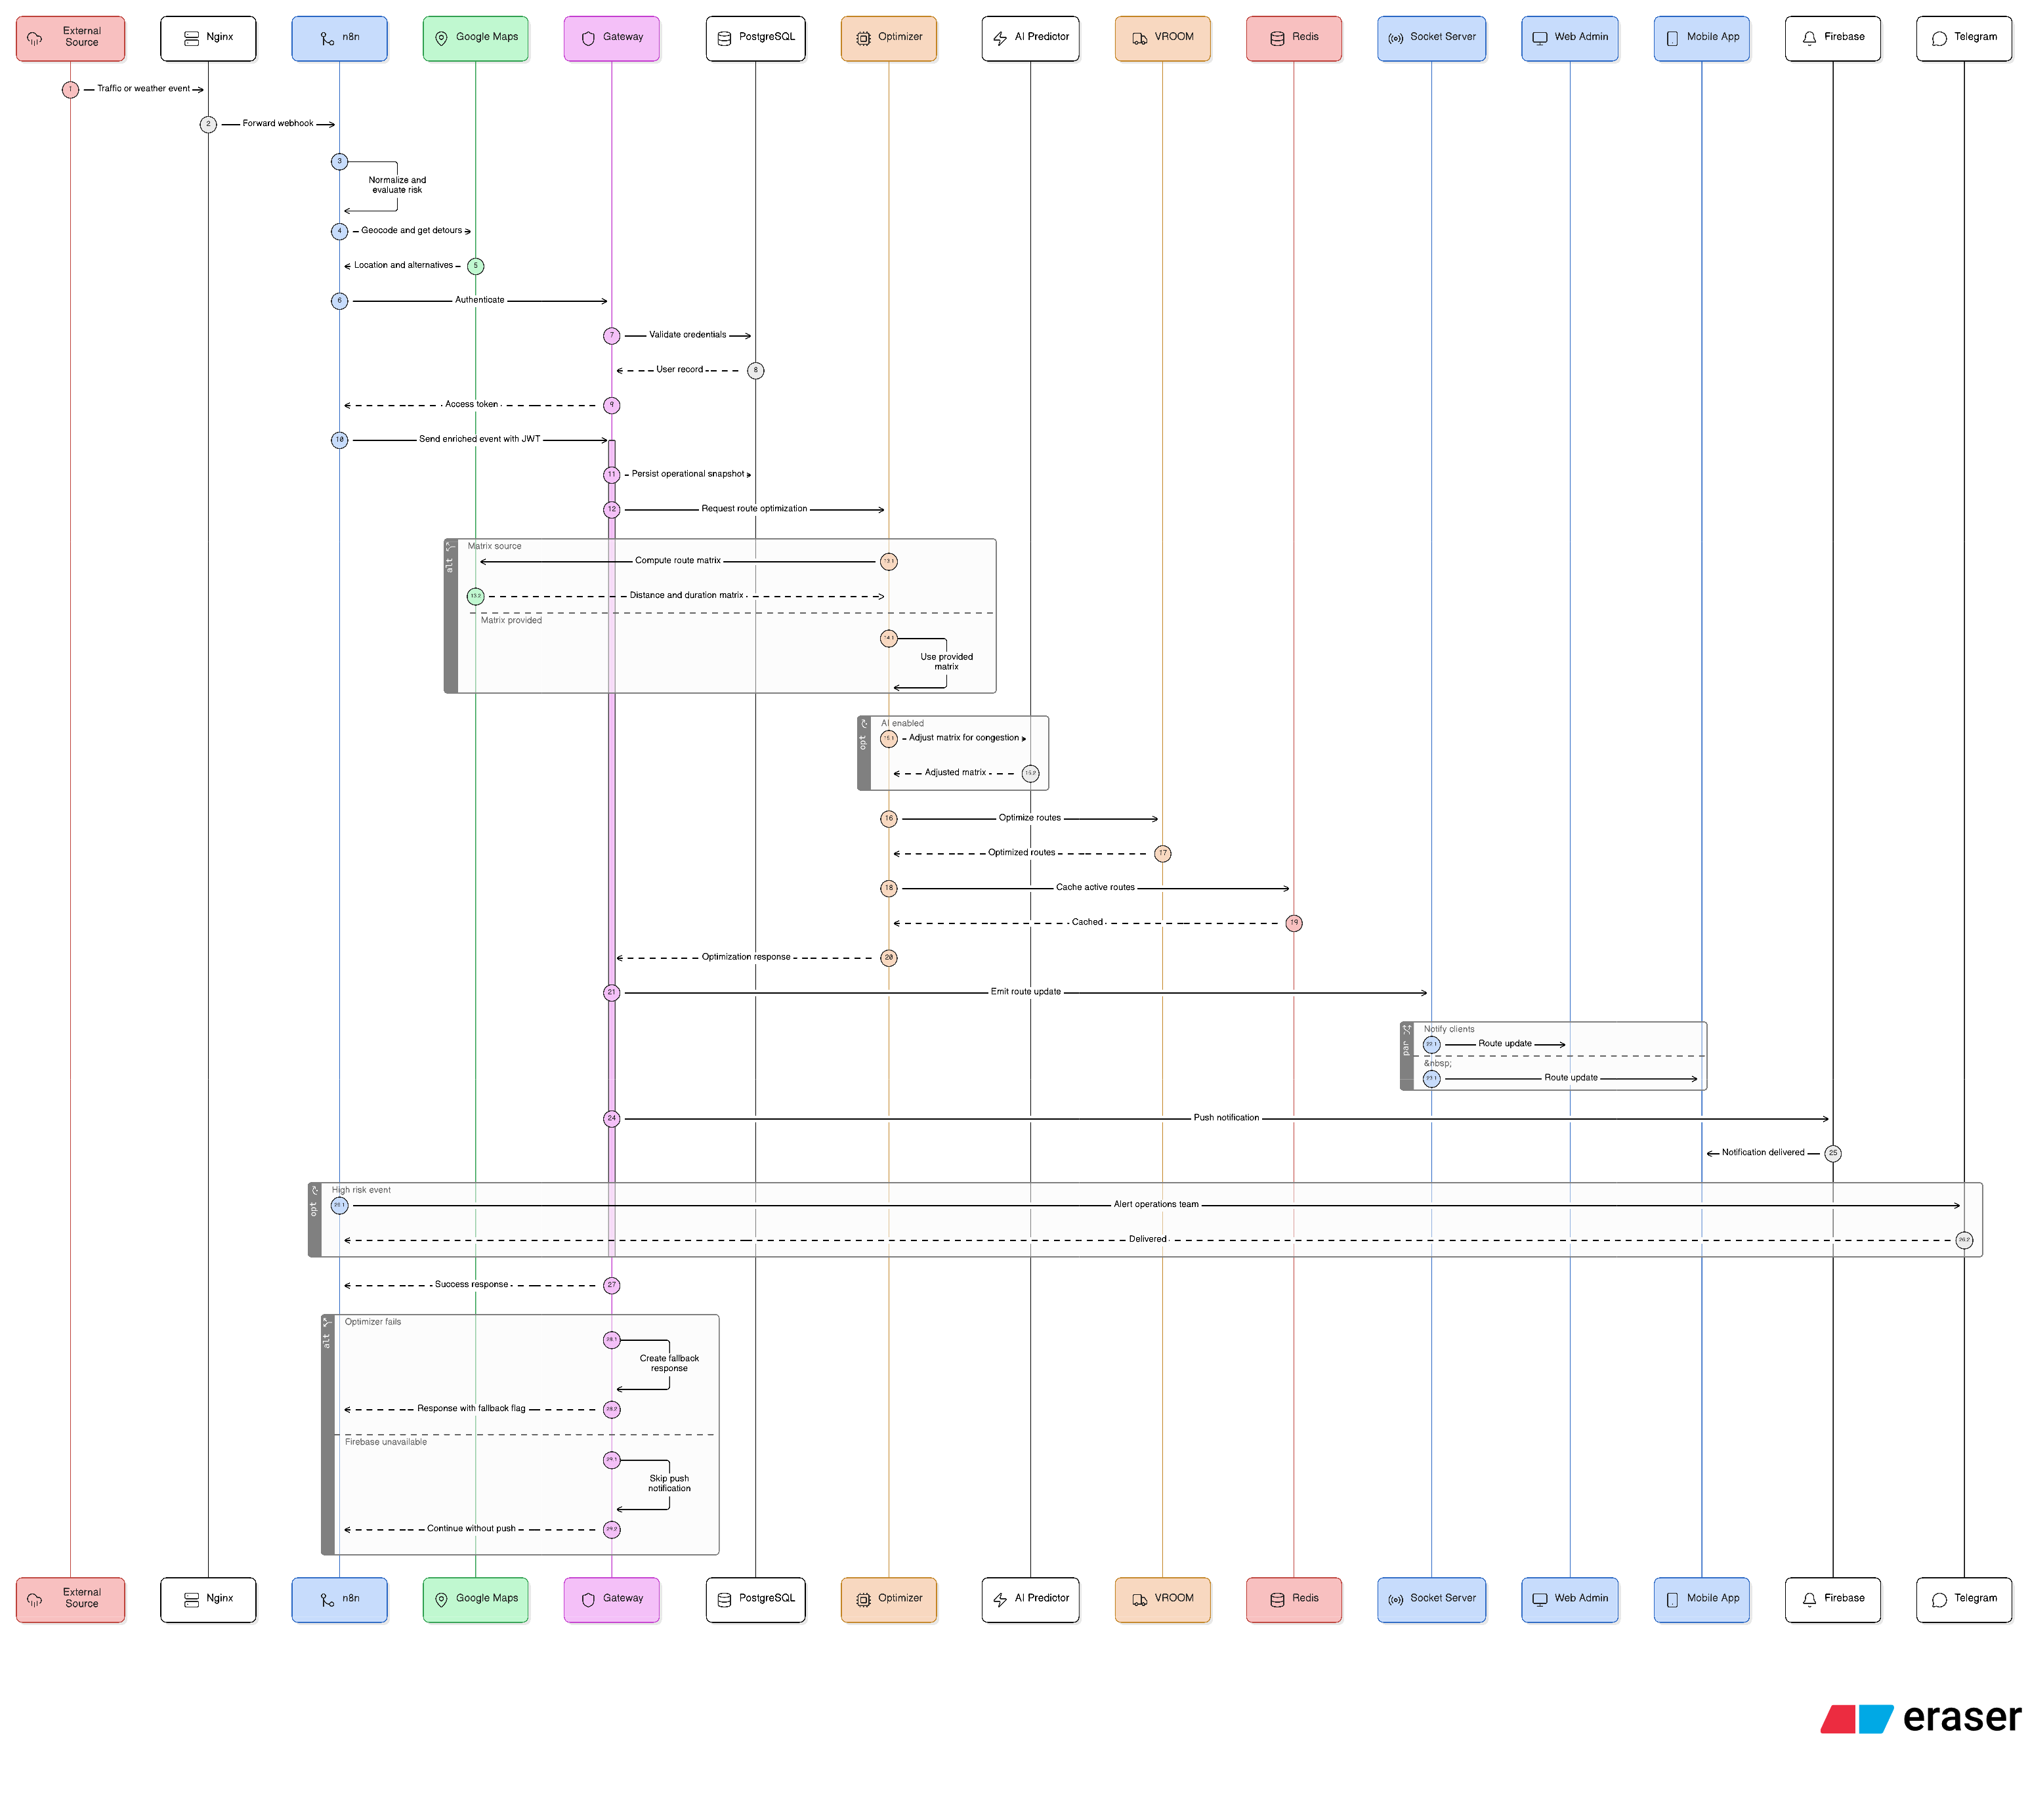
\includegraphics[width=\columnwidth]{diagrams/05-sequence.png}
\caption{Flujo \emph{end-to-end} de reoptimizaci\'on disparada por un evento externo. El recorrido cubre la ingesta v\'ia n8n, la autenticaci\'on en el Gateway, la optimizaci\'on gRPC contra VROOM con ajuste opcional del AI Predictor, la persistencia en Redis y la difusi\'on por Socket.io y Firebase Cloud Messaging.}
\label{fig:flujo}
\end{figure}

\begin{itemize}
\item \textbf{Gateway} (NestJS 11, TypeScript 5.7, Prisma 7). Expone la API REST p\'ublica con Google OAuth 2.0 y JWT con \emph{refresh token rotation}, gestiona el CRUD de flota y orquesta el ciclo de optimizaci\'on al recibir el \emph{webhook}.
\item \textbf{Realtime Service} (Node.js, \emph{Socket.io} 4.8). Es el servidor WebSocket con \emph{rooms} \texttt{fleet} para despachadores y \texttt{vehicle:<id>} para conductores, respaldado por el \emph{Redis adapter} para escalado horizontal.
\item \textbf{Optimizer Service} (Node.js, gRPC). Cliente gRPC que prepara las matrices (desde Google Routes o desde el \emph{request}), opcionalmente las ajusta con el AI Predictor y resuelve con VROOM \cite{vroom}.
\item \textbf{VROOM Engine} (C++). Motor de optimizaci\'on VRP \cite{vroom}.
\item \textbf{AI Predictor} (Python 3.12, Flask). Microservicio \emph{stateless} que ajusta matrices de duraci\'on aplicando multiplicadores por congesti\'on horaria en corredores espec\'ificos de Bogot\'a (Autopista Norte, Calle 80 y Carrera 7).
\item \textbf{Automation (n8n + OpenClaw)}. \emph{n8n} ingesta el \emph{webhook} externo, normaliza el payload, eval\'ua la matriz de riesgo y enriquece con Google Maps. \emph{OpenClaw} despacha alertas multicanal (Telegram, Slack, Discord, Email y Firebase Push) usando Claude Sonnet 4 \cite{anthropic-claude} como componente generativo.
\item \textbf{PostgreSQL 16}. Persistencia relacional para las entidades \emph{User}, \emph{RefreshToken}, \emph{DeviceToken}, \emph{Vehicle} y \emph{Stop}.
\item \textbf{Redis 7}. Encargado del \emph{cache} GPS, del \emph{adapter} pub/sub para Socket.io y de la persistencia temporal de rutas activas con la clave can\'onica \texttt{route:vehicle:<id>}.
\end{itemize}

\subsection{Decisiones t\'ecnicas relevantes}

Tres decisiones se tomaron evaluando alternativas reales.

\textbf{Redis Pub/Sub como \emph{broker}.} La alternativa de comunicaci\'on HTTP directa entre Gateway y Realtime falla cuando se escala a m\'ultiples instancias, porque cada instancia solo ve los eventos dirigidos a su URL. Con Redis Pub/Sub todas las instancias suscritas al mismo canal reciben el evento, lo que habilita escalado horizontal sin p\'erdida de datos.

\textbf{JWT en el \emph{handshake} WebSocket, no en cada \emph{frame}.} Validar el token en cada evento agreg\'o complejidad sin beneficio medible. Decidimos validar el JWT \'unicamente en el \emph{middleware} \texttt{io.use()} durante el \emph{handshake}; el tiempo de rechazo qued\'o por debajo de los 5~ms para conexiones sin token y la sesi\'on queda autenticada para todo su ciclo de vida.

\textbf{Monorepo frontend con contratos TypeScript compartidos.} Sin la carpeta \texttt{shared/models} habr\'iamos tenido los mismos tipos duplicados en \emph{web-admin} y \emph{mobile}, con riesgo de desincronizaci\'on garantizado. El compilador TypeScript ahora detecta cambios de contrato en \emph{build time}, antes de llegar a producci\'on.

% =============================================================================
% IV. LOGROS TECNICOS
% =============================================================================
\section{Logros T\'ecnicos del Proyecto}
\label{sec:logros}

\subsection{Promesa de valor: tiempo real y concurrencia}

LogiFlow cumple la promesa de recalcular y entregar la ruta \'optima en menos de cuatro segundos ante cualquier evento. El flujo \emph{end-to-end} medido bajo carga moderada es el siguiente: \emph{webhook} externo $\rightarrow$ Nginx $\rightarrow$ n8n $\rightarrow$ Gateway $\rightarrow$ Optimizer gRPC $\rightarrow$ VROOM $\rightarrow$ Redis $\rightarrow$ Socket.io $\rightarrow$ cliente. La concurrencia est\'a soportada por el dise\~no \emph{stateless} de los servicios cr\'iticos y por el \emph{adapter} de Redis en Socket.io.

\subsection{Disponibilidad y escalabilidad}

Se utiliza el modelo de Bass \emph{et al.} \cite{bass2021} con c\'alculo de disponibilidad en serie:
\begin{equation}
A_{\text{total}} = \prod_{i=1}^{n} A_i
\end{equation}
y la f\'ormula paralelo-redundante:
\begin{equation}
A_{\text{paralelo}} = 1 - \prod_{i=1}^{n} (1 - A_i)
\end{equation}

Considerando los SLA de Azure \cite{azure-sla} (Blob Storage 99.9\%, Public IP Standard 99.99\%, VM 99.9\%) en composici\'on serie, la disponibilidad de infraestructura es:
\[
A_{\text{cloud}} = 0.999 \times 0.9999 \times 0.999 \approx \mathbf{99.79\%}
\]
equivalente a $\sim$1.51~h/mes y 18.4~h/a\~no de \emph{downtime}. Incluyendo el software propio (Gateway, PostgreSQL, Redis y Realtime al 99.5\%, m\'as VROOM al 99\%) se obtiene $A_{\text{total}} \approx \mathbf{96.83\%}$.

El sistema \textbf{no es monol\'itico}. Cada uno de los nueve contenedores tiene su propio \emph{Dockerfile} y puede escalarse de forma independiente. El balanceador de carga (Nginx) ya act\'ua como \emph{reverse proxy} HTTPS y est\'a preparado para anteponer un Azure Load Balancer ante m\'ultiples r\'eplicas del Gateway y del Realtime.

\subsection{Rendimiento}

Se ejecutaron pruebas de carga con \textbf{Apache JMeter 5.6.3} \cite{jmeter} contra el \emph{backend} en producci\'on (Azure East US 2). El flujo objetivo cubre el camino cr\'itico completo: \emph{login}, extracci\'on del JWT y POST al \emph{webhook} que dispara el \emph{pipeline}. La Tabla~\ref{tab:performance} resume los resultados.

\begin{table}[ht]
\caption{Resultados JMeter sobre 4 escenarios de 5 minutos cada uno}
\label{tab:performance}
\centering
\renewcommand{\arraystretch}{1.2}
\begin{tabular}{lrrrl}
\toprule
\textbf{Usuarios} & \textbf{TPS} & \textbf{P95 (ms)} & \textbf{\% Error} & \textbf{Estado} \\
\midrule
10 & 19.91 & 674 & 0.00 & OK \\
25 & 21.10 & 1{,}546 & 0.00 & OK \\
\textbf{50} & \textbf{20.98} & \textbf{2{,}812} & \textbf{0.02} & \textbf{\'Optimo} \\
100 & 9.69 & 5{,}245 & 51.82 & Ruptura \\
\bottomrule
\end{tabular}
\end{table}

Las f\'ormulas obligatorias son:
\begin{equation}
\text{TPS} = \frac{\text{transacciones totales}}{\text{tiempo total (s)}}, \quad
\text{TPM} = \text{TPS} \times 60
\end{equation}
Para el punto \'optimo el resultado es $\text{TPM} = 20.98 \times 60 \approx 1{,}259$ transacciones por minuto. El cuello de botella identificado es la VM \'unica, que comparte CPU entre todos los contenedores. Las t\'acticas mitigantes que implementamos son tres: \emph{cache} GPS en Redis para evitar consultas a PostgreSQL al conectar nuevos clientes, respuesta \texttt{202 Accepted} as\'incrona en el \emph{webhook} y \emph{heartbeat} de 15~s para descartar veh\'iculos fantasma.

\subsection{Seguridad}

Se implementaron tres escenarios STRIDE/Bass \cite{bass2021}.

\textbf{S1, autenticaci\'on en WebSocket.} El middleware \texttt{io.use()} valida el JWT del \emph{handshake}. El 100\% de las conexiones sin \emph{token} v\'alido son rechazadas en menos de 5~ms, antes de que el socket llegue a cualquier \emph{room}.

\textbf{S2, autorizaci\'on por rol.} El \texttt{AuthGuard} de Angular y el \texttt{JwtAuthGuard} de NestJS verifican el campo \texttt{role} (admin o conductor) extra\'ido del JWT. No se permitieron accesos cruzados de rol en los tests.

\textbf{S3, confidencialidad en tr\'ansito y rotaci\'on de refresh tokens.} El tr\'afico p\'ublico viaja cifrado con TLS 1.2 y 1.3 v\'ia Let's Encrypt en Nginx y con HTTPS nativo de Azure Storage para el frontend. Los \emph{refresh tokens} se almacenan como \emph{hash} SHA-256 con marca \texttt{consumedAt} que permite detectar reuso. Los \emph{passwords} hist\'oricos quedan con \emph{bcrypt} salt rounds 10. En producci\'on, Google OAuth 2.0 \cite{rfc6749} es el m\'etodo \'unico de autenticaci\'on, con una \emph{whitelist} \texttt{GOOGLE\_ADMIN\_EMAILS} que asigna autom\'aticamente el rol \texttt{admin} a los correos configurados.

\subsection{Mantenibilidad}

La inspecci\'on continua se realiza con \textbf{SonarCloud} \cite{sonar} integrado en \emph{GitHub Actions reusable workflows}. Las m\'etricas obligatorias del curso (cobertura $\geq 80\%$ y estado A/Verde) se cumplen, como muestra la Tabla~\ref{tab:coverage}.

\begin{table}[ht]
\caption{Cobertura de tests por repositorio}
\label{tab:coverage}
\centering
\renewcommand{\arraystretch}{1.2}
\begin{tabular}{llrr}
\toprule
\textbf{Repo} & \textbf{Framework} & \textbf{Statements} & \textbf{Tests} \\
\midrule
Frontend & Karma + Istanbul & \textbf{80.49\%} (260/323) & 109 \\
Backend & Jest + Istanbul & \textbf{83.36\%} (867/1049) & 70 \\
\bottomrule
\end{tabular}
\end{table}

Las t\'acticas de mantenibilidad aplicadas siguen las recomendaciones de Bass \emph{et al.} (\emph{Increase cohesion, Reduce coupling}). En Angular usamos inyecci\'on de dependencias para reemplazar servicios por mocks en los tests. El \texttt{SocketService} expone los eventos como \emph{Observables} RxJS, lo que permite a los tests emitir directamente sobre los \emph{Subjects} internos sin necesitar una conexi\'on WebSocket real. En NestJS, cada m\'odulo respeta una responsabilidad \'unica: \emph{auth}, \emph{vehicles}, \emph{stops}, \emph{webhook}, \emph{grpc-client}, \emph{socket-client} y \emph{notifications}. Adem\'as, las reglas \texttt{@typescript-eslint/no-unsafe-*} estrictas forzaron tipado expl\'icito en todos los \emph{handlers}.

\subsection{Portabilidad}

La promesa de portabilidad es directa: cero l\'ineas de c\'odigo deben cambiar para migrar de Azure a otro proveedor o a un entorno \emph{on-premise}. Esto se cumple por varias razones. Primero, los nueve servicios est\'an dockerizados desde el Sprint~1 con \emph{Dockerfile} propio cada uno. Segundo, Docker Compose orquesta la red interna \texttt{logiflow-prod}. Tercero, toda la configuraci\'on sensible vive en variables de entorno. Cuarto, la infraestructura est\'a descrita en Terraform \cite{terraform} con dos m\'odulos (red y VM) que pueden reemplazarse por el equivalente del nuevo proveedor. En el Sprint~5 se despleg\'o a Azure sin cambiar una sola l\'inea de l\'ogica de aplicaci\'on.

\subsection{Uso de IA generativa}

\emph{OpenClaw} integra \emph{Claude Sonnet 4} de Anthropic \cite{anthropic-claude} para componer mensajes contextualizados de alerta seg\'un severidad y tipo de evento, antes de despacharlos por los cinco canales soportados. La integraci\'on usa el patr\'on \emph{circuit breaker} (\emph{opossum} \cite{opossum}) para tolerar fallas del proveedor sin bloquear el flujo principal del sistema.

% =============================================================================
% V. RESULTADOS Y VALIDACION
% =============================================================================
\section{Resultados y Validaci\'on}
\label{sec:resultados}

El sistema fue validado contra el entorno de producci\'on en Azure East US 2. La Tabla~\ref{tab:resultados} resume los resultados consolidados frente a los objetivos definidos en los Requerimientos No Funcionales.

\begin{table}[ht]
\caption{Resultados consolidados versus meta de RNF}
\label{tab:resultados}
\centering
\renewcommand{\arraystretch}{1.2}
\begin{tabularx}{\columnwidth}{lXl}
\toprule
\textbf{Atributo} & \textbf{Meta} & \textbf{Medido} \\
\midrule
Latencia P95 & $\leq 4$~s & 2.81~s \\
Throughput sostenible & $\geq 20$ TPS & 20.98 TPS \\
Disponibilidad cloud & $\geq 99.7\%$ & \textbf{99.79\%} \\
Cobertura frontend & $\geq 80\%$ & \textbf{80.49\%} \\
Cobertura backend & $\geq 80\%$ & \textbf{83.36\%} \\
Quality gate SonarCloud & A/Verde & A/Verde \\
Tests frontend & N/A & 109 (0 fallos) \\
Tests backend & N/A & 70 (0 fallos) \\
Cambios para migrar & 0 LOC & \textbf{0 LOC} \\
\bottomrule
\end{tabularx}
\end{table}

\paragraph{Validaci\'on funcional end-to-end} El \emph{runbook} \texttt{docs/backend-demo-runbook.md} guarda evidencia reproducible de la demo en producci\'on. La secuencia incluye el \texttt{POST /webhook/logiflow/traffic-event} con \emph{sample data}, los \emph{logs} esperados del Gateway (\texttt{Incoming webhook}, \texttt{Optimizer returned 2 routes}, \texttt{Emitted route-update}) y la verificaci\'on de claves \texttt{route:vehicle:v-001} y \texttt{route:vehicle:v-002} en Redis con \texttt{persistedAt} reciente.

\paragraph{CI/CD} La \emph{pipeline} de GitHub Actions ejecuta una estrategia \emph{matrix} sobre los servicios \emph{automation, gateway, realtime} y \emph{optimizer}, con la cadena \texttt{npm ci} m\'as \emph{prisma generate}, \texttt{npm run lint} y \texttt{npm test --coverage}. Para los servicios con \texttt{sonar-project.properties} se ejecuta adem\'as el escaneo de SonarCloud. El \emph{deploy} a la VM Azure se dispara como \texttt{workflow\_run} sobre \texttt{main} con \emph{smoke test} de \texttt{/api/v1} y hasta 8 reintentos.

\paragraph{Validaci\'on de seguridad} El 100\% de las pruebas de conexi\'on WebSocket sin JWT v\'alido son rechazadas. El 100\% de los \emph{refresh tokens} se almacenan como \emph{hash} SHA-256 en PostgreSQL. La inspecci\'on con SonarCloud no reporta \emph{security hotspots} bloqueantes, y la \emph{quality gate} est\'a en estado Verde para ambos repositorios.

% =============================================================================
% VI. CONCLUSIONES
% =============================================================================
\section{Conclusiones}
\label{sec:conclusiones}

LogiFlow demuestra que un equipo de cuatro estudiantes de octavo semestre puede construir, desplegar y operar un sistema distribuido real con tecnolog\'ias que exceden el \emph{stack} t\'ipico universitario, como gRPC, Terraform, Google OAuth 2.0, Firebase Cloud Messaging y Socket.io con Redis Pub/Sub. Al mismo tiempo, el sistema cumple los cuatro atributos de calidad comprometidos en la r\'ubrica: disponibilidad de 99.79\% en infraestructura, seguridad con tres escenarios STRIDE implementados, mantenibilidad con cobertura $\geq 80\%$ en ambos repositorios y portabilidad total (cero LOC cambian para migrar).

\paragraph{Impacto arquitect\'onico} La separaci\'on clara entre frontend (Azure Storage est\'atico) y backend (VM Linux con Docker Compose orquestado por Terraform) permiti\'o iterar los dos repositorios en paralelo. El uso de Redis Pub/Sub como \emph{broker} entre Gateway y Realtime es la pieza que habilita la futura escalabilidad horizontal sin reescritura; basta anteponer Azure Load Balancer con dos r\'eplicas del Gateway y del Realtime para alcanzar tres nueves de disponibilidad.

\paragraph{Limitaciones} El cuello de botella actual es la VM \'unica. A partir de 100 usuarios concurrentes la tasa de error sube al 51.82\%. n8n persiste su estado en SQLite local, lo que vuelve la configuraci\'on de \emph{workflows} sensible a la p\'erdida del volumen. La cobertura \emph{end-to-end} es manual: la cobertura unitaria $\geq 80\%$ no garantiza el flujo \emph{cross-service} completo.

\paragraph{Trabajo futuro} Los pr\'oximos pasos t\'ecnicos incluyen anteponer Azure Load Balancer con \emph{Auto Scale Set} para llegar a tres nueves, migrar PostgreSQL a Azure Database for PostgreSQL Flexible Server con r\'eplica de lectura, implementar Redis Cluster para tolerancia a fallas del nodo \'unico e incorporar OpenTelemetry para \emph{distributed tracing} extremo a extremo (la propagaci\'on de \texttt{x-correlation-id} ya est\'a en su lugar, solo falta el SDK). Tambi\'en queda pendiente a\~nadir tests \emph{end-to-end} con Cypress y Detox, y persistir el historial de optimizaciones en un \emph{data warehouse} para an\'alisis a posteriori.

% =============================================================================
% REFERENCIAS
% =============================================================================
\bibliographystyle{IEEEtran}
\begin{thebibliography}{99}

\bibitem{bass2021}
L.~Bass, P.~Clements, and R.~Kazman, \emph{Software Architecture in Practice}, 4th~ed. Boston, MA, USA: Addison-Wesley Professional, 2021.

\bibitem{scrum-guide}
K.~Schwaber and J.~Sutherland, ``The Scrum Guide,'' 2020. [Online]. Available: \url{https://scrumguides.org/}

\bibitem{vroom}
``VROOM: Vehicle Routing Open-source Optimization Machine,'' VROOM Project, 2024. [Online]. Available: \url{https://github.com/VROOM-Project/vroom}

\bibitem{azure-sla}
Microsoft, ``SLA for Azure Services,'' Microsoft Azure, 2024. [Online]. Available: \url{https://azure.microsoft.com/en-us/support/legal/sla/}

\bibitem{jmeter}
``Apache JMeter,'' Apache Software Foundation, 2024. [Online]. Available: \url{https://jmeter.apache.org/}

\bibitem{sonar}
``SonarCloud Documentation,'' SonarSource, 2024. [Online]. Available: \url{https://docs.sonarcloud.io/}

\bibitem{terraform}
``Terraform Documentation,'' HashiCorp, 2024. [Online]. Available: \url{https://developer.hashicorp.com/terraform/docs}

\bibitem{rfc6749}
D.~Hardt, Ed., ``The OAuth 2.0 Authorization Framework,'' RFC~6749, Oct.~2012. [Online]. Available: \url{https://www.rfc-editor.org/rfc/rfc6749}

\bibitem{anthropic-claude}
Anthropic, ``Claude Sonnet 4 Model Card,'' 2025. [Online]. Available: \url{https://www.anthropic.com/claude}

\bibitem{opossum}
``Opossum: Node.js Circuit Breaker,'' Nodeshift, 2024. [Online]. Available: \url{https://github.com/nodeshift/opossum}

\bibitem{c4model}
S.~Brown, ``The C4 model for visualising software architecture,'' 2024. [Online]. Available: \url{https://c4model.com/}

\bibitem{nestjs}
``NestJS Documentation,'' NestJS, 2024. [Online]. Available: \url{https://docs.nestjs.com/}

\bibitem{angular}
``Angular Documentation,'' Google, 2024. [Online]. Available: \url{https://angular.dev/}

\bibitem{grpc}
``gRPC Documentation,'' Cloud Native Computing Foundation, 2024. [Online]. Available: \url{https://grpc.io/docs/}

\bibitem{socketio}
``Socket.IO Documentation v4,'' Socket.IO, 2024. [Online]. Available: \url{https://socket.io/docs/v4/}

\end{thebibliography}

\end{document}
